\section{Metodología}
Con el fin de resolver las necesidades del ajedrez cuántico, se requiere el uso de una red neuronal que sea capaz de interpretar y utilizar los conceptos del ajedrez cuántico.

Para poder jugar de manera correcta, coherente y desafiante al ajedrez cuántico, se necesita una red neuronal que pueda calcular movimientos a partir de un estado inicial. Dicho estado es un tablero común y corriente con las piezas en él. Para alcanzar este objetivo, se ha planteado el siguiente gráfico, que representa el pipeline mediante el cual se obtendrá la data, para usarse posteriormente en el entrenamiento de la red neuronal, considerando también el ajuste de hiperparámetros mediante un algoritmo metaheurístico.

\begin{center}
    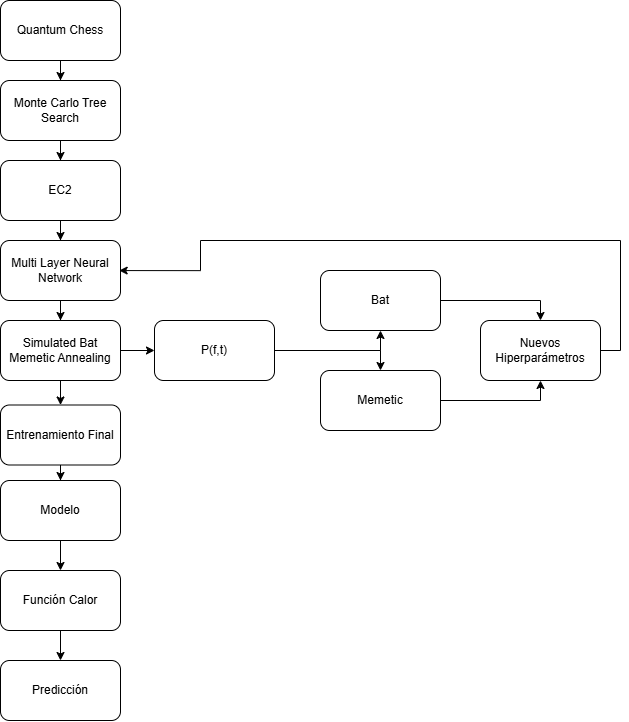
\includegraphics[scale=0.4]{Imagenes/metodologia.drawio.png}
\end{center}

A continuación, una breve descripción de cada componente desarrollado para la implementación final del juego.

\subsection{Quantum Chess}

Sobre él se juegan las partidas, también se le puede llamar entorno de juego. Tiene implementadas tanto las reglas del juego tradicional, como las reglas de la mecánica cuántica para hacerlo un juego más interesante. Además, ya contiene el tablero y las piezas necesarias para poder desarrollar todas las simulaciones posibles, y también para que pueda ser jugado por una persona común.

Los movimientos especiales con mecánica cuántica que se emplearon, son los siguientes:

\subsubsection{Movimiento}

Para poder trabajar el movimiento convencional que implica cambiar la posición de una pieza entera, o una superposición de esta misma a otra, se utilizó la compuerta iSWAP, que se debe aplicar entre los dos qubits que intercambiarán valores.

Esta compuerta intercambia el valor de un qubit con otro al colapsar el circuito completo, lo cual se debe a la matriz que representa la compuerta matemáticamente.


\[
U_{iSwap} = \begin{pmatrix}
1 & 0 & 0 & 0 \\
0 & 0 & i & 0 \\
0 & i & 0 & 0 \\
0 & 0 & 0 & 1
\end{pmatrix}
\]

Se utiliza esta porque es más sensible a los patrones de memoria y puede aprender de manera más segura los patrones del circuito y así se evitan swaps inefectivos que dejarían el juego injugable por la aleatoriedad.

\subsubsection{Split} 

Para poder realizar una superposición entre dos posiciones, se debe de mantener el uso de la compuerta previamente analizada, pero esto sería únicamente para uno de los dos destinos que implican el split. El otro destino debe verse evaluado mediante sqrt(iSWAP), entre este y el mismo origen.\newline
Esta raíz sobre la compuerta, efectúa una superposición que implica que más adelante cuando se realice el colapso, existirán un 0.5 de probabilidades que aparezca en una posición u otra. Cuantos más splits haya, se irán reduciendo las probabilidades de manera lineal al respecto de cada split o slide realizado.

\[
U_{\sqrt{i\text{SWAP}}} = \begin{pmatrix}
1 & 0 & 0 & 0 \\
0 & \frac{1}{\sqrt{2}} & \frac{i}{\sqrt{2}} & 0 \\
0 & \frac{i}{\sqrt{2}} & \frac{1}{\sqrt{2}} & 0 \\
0 & 0 & 0 & 1
\end{pmatrix}
\]

\subsubsection{Slide}

El slide implica que se realice un movimiento atravesando a una pieza y pasando sobre ella como si no estuviera. Para poder hacer uso de esta regla, la pieza que será obviada, debe de encontrarse en alguna superposición. Y la compuerta que maneja este proceso, es el Controlled-iSWAP, y se tendrá que aplicar como controlador a la casilla que será atravesada, para sí en caso sea cero se tome en cuenta ese movimiento como válido, mientras que se la pieza controladora se mantuvo ahí al colapsar; el movimiento se invalide por completo.

\[
U_{\text{slide}} = \begin{pmatrix}
1 & 0 & 0 & 0 & 0 & 0 & 0 & 0 \\
0 & 0 & i & 0 & 0 & 0 & 0 & 0 \\
0 & i & 0 & 0 & 0 & 0 & 0 & 0 \\
0 & 0 & 0 & 1 & 0 & 0 & 0 & 0 \\
0 & 0 & 0 & 0 & 1 & 0 & 0 & 0 \\
0 & 0 & 0 & 0 & 0 & 1 & 0 & 0 \\
0 & 0 & 0 & 0 & 0 & 0 & 1 & 0 \\
0 & 0 & 0 & 0 & 0 & 0 & 0 & 1 \\
\end{pmatrix}
\]

\subsubsection{Split-Slide}

Para poder realizar un split-slide, se optó por utilizar una combinación de compuertas. Es decir, se realizará un Controlled-iSWAP entre la posición y su destino con slide. Luego, en caso de que no haya otro slide, se realizará un $\sqrt{iSWAP}$ hacia la dirección sin mayor problema. En caso de que sea un slide en la misma dirección, se realizará un $\sqrt{iSWAP}$, pero tomando como inicio el qubit donde se realizó inicialmente el Controlled-iSWAP. Y, por último, en caso de que se vaya en dos direcciones distintas y ambas requieran slide, a la segunda se le realizará un $\sqrt{Controlled-iSWAP}$ desde el mismo qubit de origen.

\subsubsection{Merge}
Es solo un movimiento que, a nivel lógico, permite que se encuentre en esa posición, mas no a nivel matemático, porque luego, cuando se realice el colapso, el circuito generado simulará todo y, como ese resultado comenzó a moverse junto, no importa de dónde llegue; lo que importa es que, por un lado u otro, se mantendrá el camino. La compuerta utilizada será un Controlled-iSWAP, para que si un resultado tiene 0, el otro se lo envíe, y si este tiene 0, su contraparte se lo envíe.

\subsection{Montecarlo Tree Search}
Cumple la función de jugar de manera aceptable el juego. No obstante, se tendrá que limitar tanto su ramificación como su longitud de simulación, debido a la cantidad exorbitante de movimientos posibles a partir de un estado.

El algoritmo de monte carlo utilizará como función objetivo la menor cantidad de movimientos para poder ganar la partida. No obstante, también se hará uso de una heurística, esto porque aparte de guiar el camino para la solución; como muy probablemente el árbol no pueda llegar a simular hasta tener el coste total, entonces la heurística al ser optimista llevará por caminos, según su propiedad.\newline

$h1(n)$ = Puntaje del jugador en base al valor de cada pieza.\\

$c$ = Coste (Cantidad de jugadas hasta el jaque mate)

\begin{enumerate}
    \item \textbf{Admisibilidad}: La heurística resulta admisible porque relaja el problema. Ya no busca realizar jaque mate que puede resultar complejo, comenzará a buscar la mayor puntuación que implica solo comer las más valiosas posibles.
    \item \textbf{Consistencia}: Es consistente, porque conforme se tengan más sucesores, estos siempre resultan más sencillos debido a la cantidad de puntaje reducido.
\end{enumerate}

En base a lo que pueda jugar el algoritmo, se le pondrá como contrincante otro igual para que así simulen partidas; y como el algoritmo buscará el mejor movimiento posible, entonces de esta manera se nos proveerá de data útil para la red neuronal, cosa que realizando partidas con personas resultaría tanto más costoso, como no necesariamente valioso, porque estas personas pueden cometer errores graves. Se simularán algunas partidas, pero también se generarán estados aleatorios a los que el algoritmo MCTS tendrá que darles solución, y en base a esta se generarán los datasets.

\subsection{Dataset Generado}

El dataset que se genere a partir de las partidas de Monte Carlo, consistirá en dos vectores. El primero será el tablero de ajedrez que tendrá identificada cada pieza con un número y un signo, además de un valor que indicará a quién le toca jugar.\newline
Si bien el algoritmo MCTS está desarrollado en un archivo \textit{.ipynb}; la generación y la simulación de todas las jugadas para la generación de datos, se realizan en una instancia de Amazon Linux en la plataforma AWS (Amazon Web Services), con un archivo \textit{.py.}

\subsubsection{Instancia EC2}

Las especificaciones de la instancia generada son:
\begin{itemize}
    \item \textbf{Nombre:} MCTS.
    \item \textbf{SO:} Linux.
    \item \textbf{Distribución:} Amazon Linux.
    \item \textbf{AMI:} Amazon Linux 2023 AMI 2023.6.20241121.0 x86\_64 HVM kernel\-6.1
    \item \textbf{Arquitectura:} 64 bits (x86).
    \item \textbf{Tipo de instancia:} c5ad.large - 2 vCPU (3.3 GHz) - 4 GiB RAM - 75 GiB SSD NVMe.
    \item \textbf{Almacenamiento:} 20 GiB - gp3.
\end{itemize}

Se seleccionó la distribución de Amazon Linux, ya que resulta más liviana en comparación a distribuciones más conocidas y populares como Ubuntu. Además, está optimizada para operaciones de cómputo grandes en el servicio EC2.\newline
El tipo de instancia, se seleccionó bajo el mismo criterio de soporte para un cómputo pesado, esto bajo las limitaciones del laboratorio de AWS Academy.

\subsubsection{Entrada}

{\footnotesize
\begin{tabular}{|m{1.5cm}|m{1cm}|m{1.2cm}|m{1cm}|m{2cm}|}
\hline
\textbf{Pieza} & \textbf{ID} & \textbf{Color Blanco} & \textbf{Color Negro} & \textbf{Valor en Vector} \\ \hline
Torre & 82 & 1 & -1 &  Identificador * Color \\ \hline
Caballo & 75 & 1 & -1 & Identificador * Color \\ \hline
Alfil & 66 & 1 & -1 &  Identificador * Color \\ \hline
Reina & 81 & 1 & -1 &  Identificador * Color \\ \hline
Rey & 69 & 1 & -1 & Identificador * Color \\ \hline
Peon & 80 & 1 & -1 & Identificador * Color \\ \hline
Espacio en Blanco & 0 & 0 & 0 & 0 \\ \hline
\end{tabular}
}\newline

Y con estos valores, el tablero que se tenga en base a strings se convertirá en un arreglo numérico basado en el diccionario previamente establecido.\newline
Con respecto al output para predecir, se utilizará de igual manera un vector. Este indicará:

$v = (\text{Movimiento}, \text{Origen} 1, \text{Origen} 2, \text{Destino} 1, \text{Destino} 2,\newline \text{Coronación})$

Y los valores establecidos para cada uno de los parámetros del vector son:

\subsubsection{Salida}
\paragraph{Movimiento}
\begin{center}
\begin{tabular}{|c|c|}
\hline
\textbf{Movimiento} & \textbf{Valor} \\ \hline
Basico & 1\\ \hline
Split  & 2 \\\hline
Swap   & 3 \\\hline
\end{tabular}
\end{center}
Para el movimiento no se toma en cuenta el slide, ya que, está implícito dentro de cualquier movimiento, menos el merge.

\paragraph{Orígenes y destinos}
\begin{center}
\begin{tabular}{|c|c|c|}
\hline
\textbf{Valor} & \textbf{Necesita movimiento} & \textbf{No necesita} \\ \hline
Origen 1    & Valor de 0 a 63 & -\\ \hline
Origen 2    & Valor de 0 a 63 & -1\\\hline
Destino 1   & Valor de 0 a 63 & -\\\hline
Destino 2   & Valor de 0 a 63 & -1\\\hline
\end{tabular}
\end{center}
\paragraph{Coronación}
\begin{center}
    \begin{tabular}{|c|c|}
    \hline
    \textbf{Pieza} & \textbf{Valor} \\ \hline
    No hay Coronación & 0\\ \hline
    Torre  & 1 \\\hline
    Reina   & 2 \\\hline
    Alfil   & 3 \\\hline
    Caballo   & 4 \\\hline
    \end{tabular}    
\end{center}

La data no llevará un tratamiento especial, ya que, como es generada por el computador, esta ya está completa y es fiable por el algoritmo que la generó.

\subsection{Multi Layer Neural Network with Output Heads}

Tras conseguir de las simulaciones con Monte Carlo datos de entrenamiento. Estos se procederán a utilizar como input a la red neuronal.\newline
Para el proceso de entrenamiento se tomarán los datos con un 25\% que será para el test, mientras que un 75\% para el train. De esta forma se podrá ver si las jugadas que realizará el modelo tienen relación con lo que aprendió y si realmente está trabajando bajo la misma lógica de Monte Carlo para llegar a las mismas conclusiones sobre qué movimientos realizar. Prácticamente es una regresión con respecto a MCTS.\newline
La red neuronal multicapa se encargará de mejorar el proceso de aprendizaje, ya que, pasará por capas de neuronas, para así ajustar a cada parámetro de salida necesario de manera más óptima. Todo esto para que finalmente, en la última capa se le asignen distintos cabezales de salida (uno para cada output del vector planteado); se toma esta metodología para poder dar predicciones con valores de entre cero y uno para cada componente del vector resultado, aplicando softmax a cada cabezal independiente del otro (para eso el uso de cabezales de salida). Esto es porque como el resultado de la predicción no necesariamente es buena o mala respecto a la entrada, si se le asignara a predecir valores directamente existiría un sesgo en base a la distancia entre los resultados en el espacio; cosa que no aplica para el caso porque no necesariamente existirá un resultado mejor o peor, solo lo más aproximado a como jugaría MCTS.\newline
La cantidad de neuronas por capas, y todos las funciones de activación por estas, se inicializarán aleatoriamente, pero según la bibliografía estudiada para el apartado de la profundidad, ya luego se irán ajustando con el uso del Bat Algorithm y Memetic Algorithm usando la metodología del Simulated Annealing Algorithm.\newline
Finalmente, cuando se compruebe que la red puede predecir movimientos del algoritmo Monte Carlo, entonces se pondrá a prueba en juegos y matrices de confusión para ver su funcionamiento.

\subsection{Hybrid Algorithm}
Se plantea un algoritmo híbrido que combina tres metaheurísticos para conseguir la mejor optimización de los hiperparámetros (neuronas por capa). De estos tres, se tomará uno que hará el papel de "switcher" para ocasionar el intercambio del uso entre los otros dos; así se logrará conseguir lo mejor del Bat Algorithm y el Memetic Algorithm.
\subsubsection{Simulated Bat Memetic Annealing (SBMA) Algorithm}
Este metaheurístico se encargará, mediante una variable de calor, ir intercambiando entre los algoritmos. Además, se tendrá en cuenta el fitness que genera cada uno de estos, ya que, su objetivo es de; si un algoritmo está dando muy buenos resultados, entonces lo normal sería que se mantenga mejorando mediante el ya seleccionado. Pero mediante la lógica del Simulated Annealing, y su variable de calor; para darle más explosividad y asegurar la mejora absoluta de resultados, se realizará el intercambio. Esto para evitar sesgos por el uso constante de un mismo algoritmo bajo sus propios parámetros optimizados.\newline

La función que realizará de calcular la probabilidad de intercambio es
$P(f,T) = 1 - \dfrac{1}{1+\alpha\times T\times(1-f)}$, donde:

\begin{itemize}
    \item $P =$ Probabilidad de salto.
    \item $f =$ Fitness actual.
    \item $T =$ Temperatura actual.
    \item $\alpha =$ Constante reguladora para ajustar limites. Usamos el valor 10.
\end{itemize}

%IMAGEN
\begin{center}
    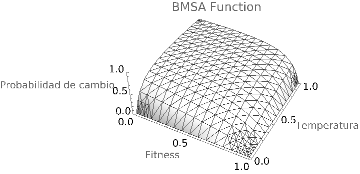
\includegraphics[scale=0.4]{Imagenes/BMSA.png}
\end{center}

Por otro lado ambos metaheurísticos, tendrán la misma función de fitness; esta función es $Fo(m,t)=\dfrac{m}{1+\alpha t}$

\begin{itemize}
    \item $Fo =$ Fitness.
    \item $m =$ 1-MAE del modelo
    \item $t =$ Tamaño normalizado en MB del modelo.
    \item $\alpha =$  Proporción de importancia del tamaño de la red. Implementado con 0.05.
\end{itemize}

El algoritmo en cuestión presenta la siguiente estructura:

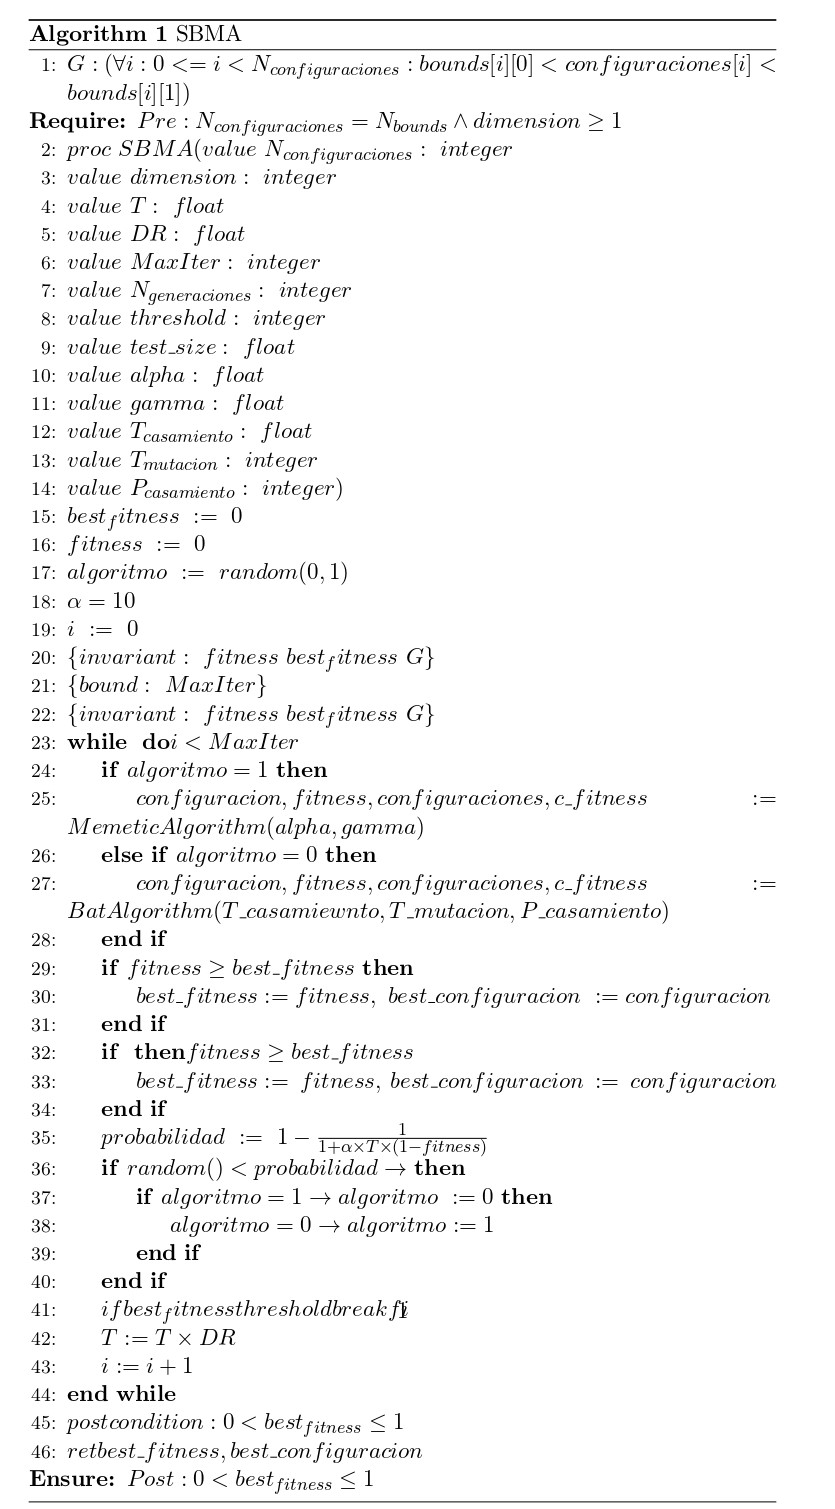
\includegraphics[scale=0.65]{Imagenes/first_pseudocode.jpg}

Otra forma de entenderlo es:
\begin{center}
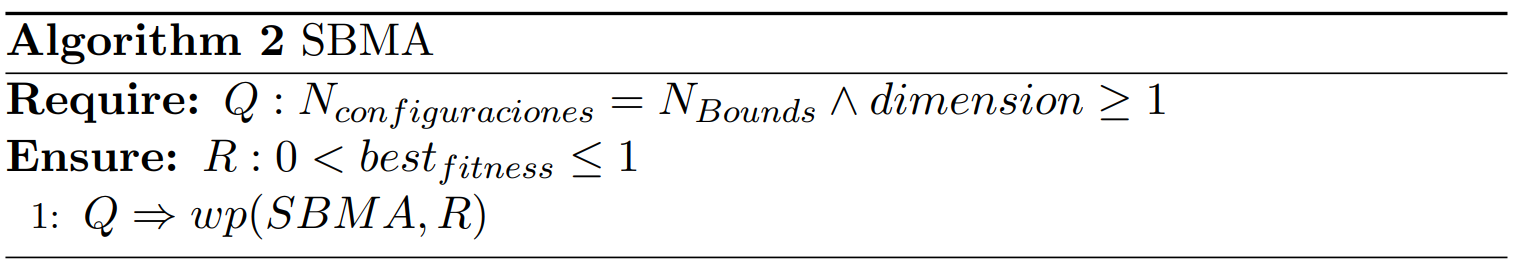
\includegraphics[scale=0.2]{Imagenes/second_pseudocode.png}
\end{center}
\subsection{Bat Algorithm}
Se basa en la ecolocalización de los murciélagos para así, poder llegar a la solución más óptima, esto porque mediante la técnica previamente mencionada se llaman unos a otros y comienzan a viajar a ciertos puntos para conseguir la mejor solución. En este caso, sería la cantidad de neuronas por capa. Este algoritmo proporcionará la explotación al SBMA, como únicamente se encarga de ajustar velocidades y puntos de cada murciélago; mejorará ese conjunto de soluciones lo más posible en base a un mejor local.

\subsection{Memetic Algorithm}

Se basa en la evolución muy similar a los algoritmos genéticos evolutivos. Con la diferencia en que, para mantener una población mínima y constante, siempre se elimina a toda la mayoría de esta bajo cierto nivel de aleatoriedad, pero siempre dando mayor prioridad de eliminación a los que presentan peores resultados. Se mantiene la mutación y reproducción entre cromosomas. Este algoritmo proporcionará la exploración al SBMA, como va generando nueva población y deshaciéndose de la peor, si bien mantiene explotación por ese lado; su punto fuerte es la exploración en la búsqueda de nuevos posibles individuos.

\subsection{Greedy Search}
Se programó el Greedy Search para poder comparar el desempeño del algoritmo híbrido con este, ya que, se considera un estándar en la optimización de hiper parámetros.
No obstante, se modificó la inicialización de datos, ya que, no partirá de entradas dadas por el usuario, sino las generará aleatoriamente para proporcionarle algo más de explotación, y ya luego se ajustará sin problemas probando las combinaciones respectivas.

\subsection{Despliegue}
El uso de la red neuronal será únicamente para sus pesos, para poder predecir, a partir de un tablero dado, qué movimiento realizar. Para esto, se realizará un despliegue dentro de Python para que se pueda jugar con un tablero elaborado en Pygame; la metodología de juego será por turnos, donde empezará el jugador con las blancas y la red neuronal será las negras, o como lo seleccione el usuario.\newline
Además, se plantea el uso de "temperatura" en las predicciones para poder variar los resultados y evitar jugar siempre de la misma manera; en caso haya una predicción errónea que contraiga un movimiento imposible, se volverá a predecir hasta llegar a una solución permitida. En caso de fallar muchas veces, se procederá a tomar una decisión aleatoria, pero se irán guardando componentes coherentes para que la aleatoriedad únicamente afecte a ciertas partes del vector de movimiento, y no sea una decisión completamente aleatoria.


\subsection{Función de calor}

Su función será generar probabilidades para poder tomar otras posibles soluciones, similarmente buenas a la mejor encontrada. Esto debido a que, la probabilidad de seleccionar una de ellas, es directamente proporcional, al porcentaje predicho por la red neuronal. Para cada probabilidad de seleccionar un resultado en el arreglo de estos, se le aplicará la función:

$P(L_i,T) = \frac{e^{\frac{L_i}{T} - max(\frac{L}{T})}}{\sum_{i=1}^{n} (e ^{ \frac{L_i}{T} - max( \frac{L}{T}) })}$, donde:

\begin{itemize}
    \item \textbf{P = } Nueva probabilidad
    \item \textbf{L = } Todas las predicciones originales de la red
    \item \textbf{$L_i$= } Indica una predicción de todas
    \item \textbf{T = } Temperatura
\end{itemize}
